\documentclass{beamer}
\usepackage[size=custom, width=121.9, height=91.44, scale=1.5, debug]{beamerposter} 
%\usepackage[size=custom, width=48in, height=36in, scale=1.4, debug]{beamerposter} 

\usetheme{Lankton}

\usepackage{amsmath, amsthm, amssymb, latexsym}
\usepackage[utf8]{inputenc}
\usepackage[T1]{fontenc}
\usepackage{mathpazo}
\usepackage[scaled=0.95]{berasans}
\usepackage[english]{babel}
\usepackage{graphicx}
\usepackage{float}
\usepackage{caption}

\graphicspath{{img/},{plots/}}

\title{Ice retreat timing and bedrock erosion of the\\Puget Lobe of the Cordilleran ice sheet}
\newcommand{\footleft}{depts.washington.edu/cosmolab}
\newcommand{\footright}{zploskey@uw.edu}
\author{Zach Ploskey and John Stone}
\institute{Cosmogenic Nuclide Lab, Dept. of Earth and Space Sciences, University of Washington, Seattle}
\date{Aug. 8th, 2014}

\begin{document}

\begin{frame}{}\centering

\begin{columns}[T]

\begin{column}{0.32\columnwidth}

\begin{block}{Overview}	
During the Frasier glaciation, ice from the Cordilleran ice sheet flowed south from Canada across the San Juan Islands and into the Puget Lowland.
This ice lobe, known as the Puget Lobe, reached its maximum extent in the Puget Lowland 16.95 cal. ka ago  (Porter and Swanson, 1998), and began to retreat within a few hundred years.

\begin{figure}
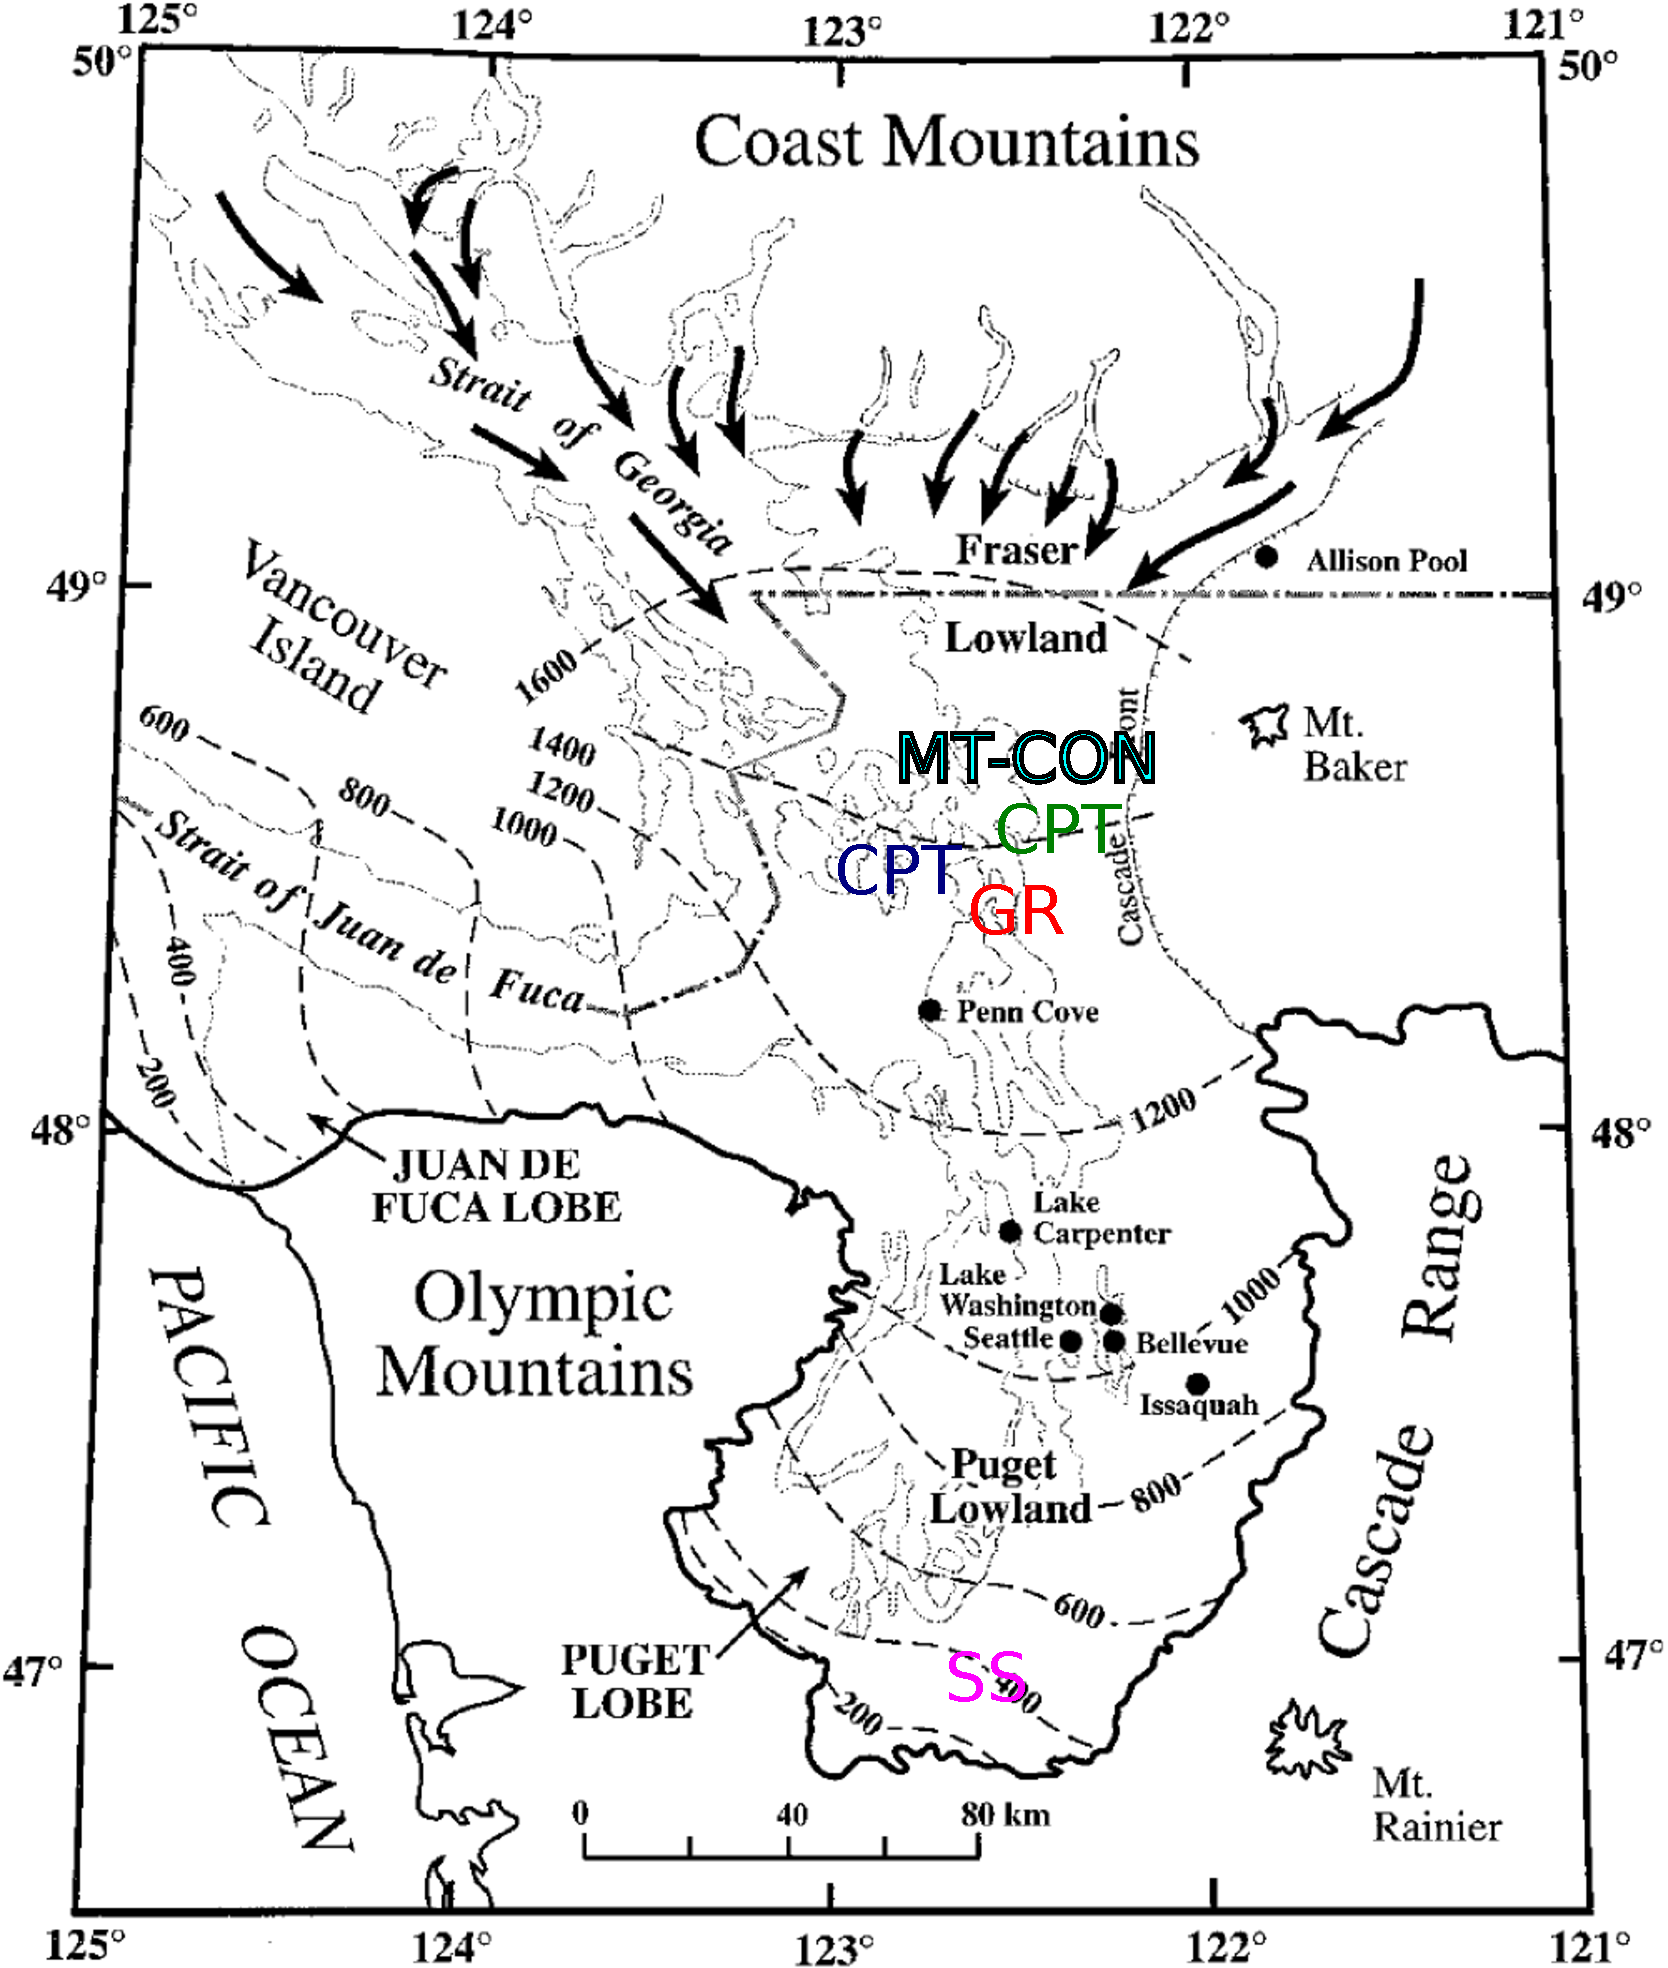
\includegraphics[width=0.6\textwidth]{lobe_map.pdf}
\caption*{Puget Lobe maximum extent (Porter and Swanson, 1998).}
\end{figure}

\end{block}

\begin{block}{Methods}
\begin{itemize}
\item We collected and measured cosmic ray-produced $^{10}$Be in glacial erratics and glacially eroded bedrock samples from the Puget Lowland and the San Juan Islands.
\item Measured $^{10}$Be concentrations in these rocks can be used to calculate exposure ages, and in the case of bedrock samples, infer the extent of erosion by glacial ice.
\item We compare the $^{10}$Be chronology to existing $^{14}$C dates from the Puget Lowland (Porter and Swanson, 1998).
\item Analyses predating the existing $^{14}$C chronology are instances of limited erosion, resulting in anomalously high concentrations and apparent exposure ages.
\item Reduced apparent exposure ages indicate shielding due to isostatic rebound, soil, sediment or tree cover.
\item Dates calculated using CRONUS Calculator 2.2 (Balco) with production rate from the UW-Scotland-CRONUS calibration data set.
\end{itemize}
\end{block}

\end{column}
	
\begin{column}{.32\columnwidth}

\begin{block}{Apparent exposure ages}
\begin{figure}
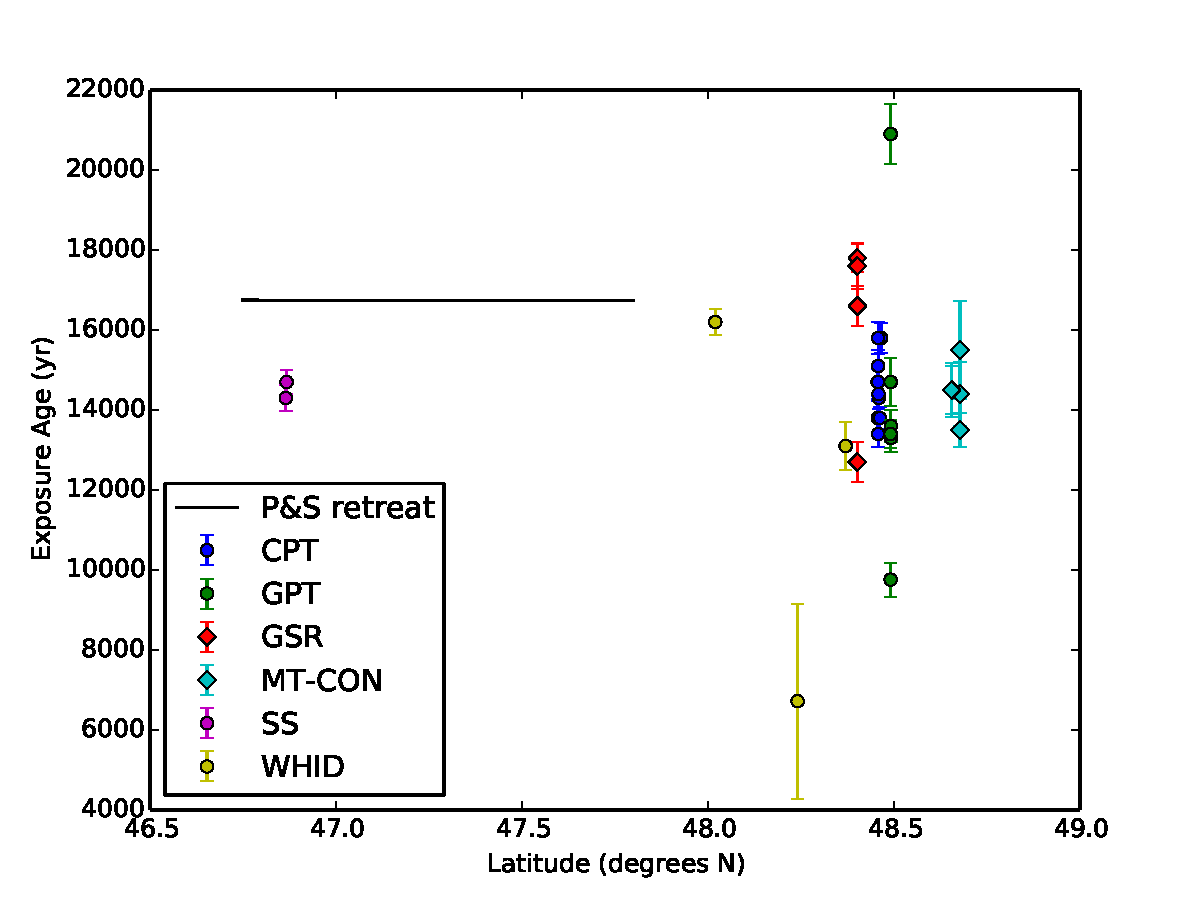
\includegraphics[width=\textwidth]{age_vs_latitude}
\end{figure}

\begin{itemize}
\item Black line shows radiocarbon-constrained retreat margin from Porter and Swanson (1998).
\item Bedrock data are plotted as diamonds.
\item All data above P\&S retreat curve must have been exposed to cosmic radiation during the previous interglacial period.
\end{itemize}

\end{block}

\begin{block}{Goose Rock (GR)}
\begin{itemize}
\item Bedrock samples from Goose Rock, north end of Whidbey Island, yield apparent exposure ages older than downstream radiocarbon dates, which would require limited glacial erosion (likely $<2$ m) of the landform during the last glaciation.
\item Two overprinted sets of glacial striations preserved at Goose Rock may be related to a brief re-advance of the ice sheet after calving retreat when it became grounded at Penn Cove, central Whidbey Island.
\item Further exposure dating of erratic boulders or radiocarbon dates from Penn Cove are needed to test this hypothesis. 
\end{itemize}	
\end{block}

\end{column}

\begin{column}{.32\columnwidth}

\begin{block}{Mt. Constitution (MT-CON)}
Bedrock samples collected further north, on Mt. Constitution, eastern Orcas Island, showed no prior exposure in a 5-sample north-south transect across the mountain. Exposure ages are consistent with an ice-free Mt. Constitution by ~14.5 ka. 
This postdates radiocarbon dates from Lake Carpenter and is consistent with upper limiting terrestrial $^{14}$C dates of 14.1 cal. ka on the Sumas I drift located upstream in the Frasier Lowland (Kovanen 2002).
\end{block}


\begin{block}{South Sound (SS) forest shielding}
\begin{itemize}
\item Large glacial erratic boulders in the southern Puget Lowland, near the ice sheet terminus, greatly underestimate the true exposure age, possibly due to heavy shielding from cosmic radiation in thick forest (Bretz, 1913).
\item With independent age constraints, cosmogenic isotope measurements from these samples could be used to estimate forest canopy biomass following deglaciation.
\item Southern Puget Sound samples have apparent exposure ages that underestimate the true deglaciation age by 8\%, which is comparable to the $7\pm2\%$ shielding factor calculated for dense Olympia forest by Plug et al. (2007).
\end{itemize}
\end{block}

\begin{block}{Conclusions}
\begin{itemize}
\item Shielding of south Sound samples is consistent with forest comparable to the Olympic rainforest at the samples sites prior to western settlement.
\item Ice retreated north of the San Juan islands by 14.5 ka.
\item Exposure of bedrock at Goose Rock, northern Whidbey Island, has not been significantly eroded for two or more interglacial periods.
\end{itemize}
\end{block}

\begin{block}{References} 
\begin{itemize}
{\tiny

\item Balco, G., Stone, J., Lifton, N., Dunai, T., 2008. A simple, internally consistent, and easily accessible means of calculating surface exposure ages and erosion rates from Be-10 and Al-26 measurements. \emph{Quat. Geochron.} 3, 174--195.

\item Bretz, J.H., 1913. Glaciation of the Puget Sound Region. \emph{Washington Geol. Survey Bull.} 8, 244 pp.

\item Kovanen, D.J. (2002). Morphologic and stratigraphic evidence for Allerød and Younger Dryas age glacier fluctuations of the Cordilleran Ice Sheet, British Columbia, Canada and northwest Washington, USA. \emph{Boreas}, 31(2), 163--184.

\item Porter, S.C., Swanson, T.W., 1998. Radiocarbon Age Constraints on Rates of Advance and Retreat of the Puget Lobe of the Cordilleran Ice Sheet during the Last Glaciation. \emph{Quat. Res.} 50, 205--213.

\item Plug, L.J., Gosse, J.C., McIntosh, J.J., Bigley, R., 2007. Attenuation of cosmic ray flux in temperate forest. \emph{J. Geophys. Res.} 112, F02022.

} %small
\end{itemize}

\end{block}

\begin{block}{Code and Data Repository}
\center \url{github.com/zploskey/puget_lobe_amqua_2014_poster}

\includegraphics{CC-BY.png}
\end{block}

\end{column}

\end{columns}

\end{frame}

\end{document}